\appendix
\chapter*{Appendices}
\addcontentsline{toc}{chapter}{Appendices}
\renewcommand{\thesection}{\Alph{section}}

\section{XDC constraints}
\label{appendix:constraints}

Using the BEL constrain, the exact \acrshort{lut} of a \acrshort{clb} can be specify for a given part of the \acrshort{tero} cell. Additionally, the PIN LOCK constrain provides control on the exact pin of the \acrshort{lut} used for a given signal. Those two constrains can help to build \acrshort{tero} cells that are identical.

On figure~\ref{fig:locked_improvement_tero_8}, we can observe the impact of those constrains on uniformity and reliability for a given device. The red points correspond to the design without the BEL and PIN LOCK constrains while the black one used both of them.

\begin{figure}[H]
   \begin{minipage}[b]{0.50\linewidth}
      \centering 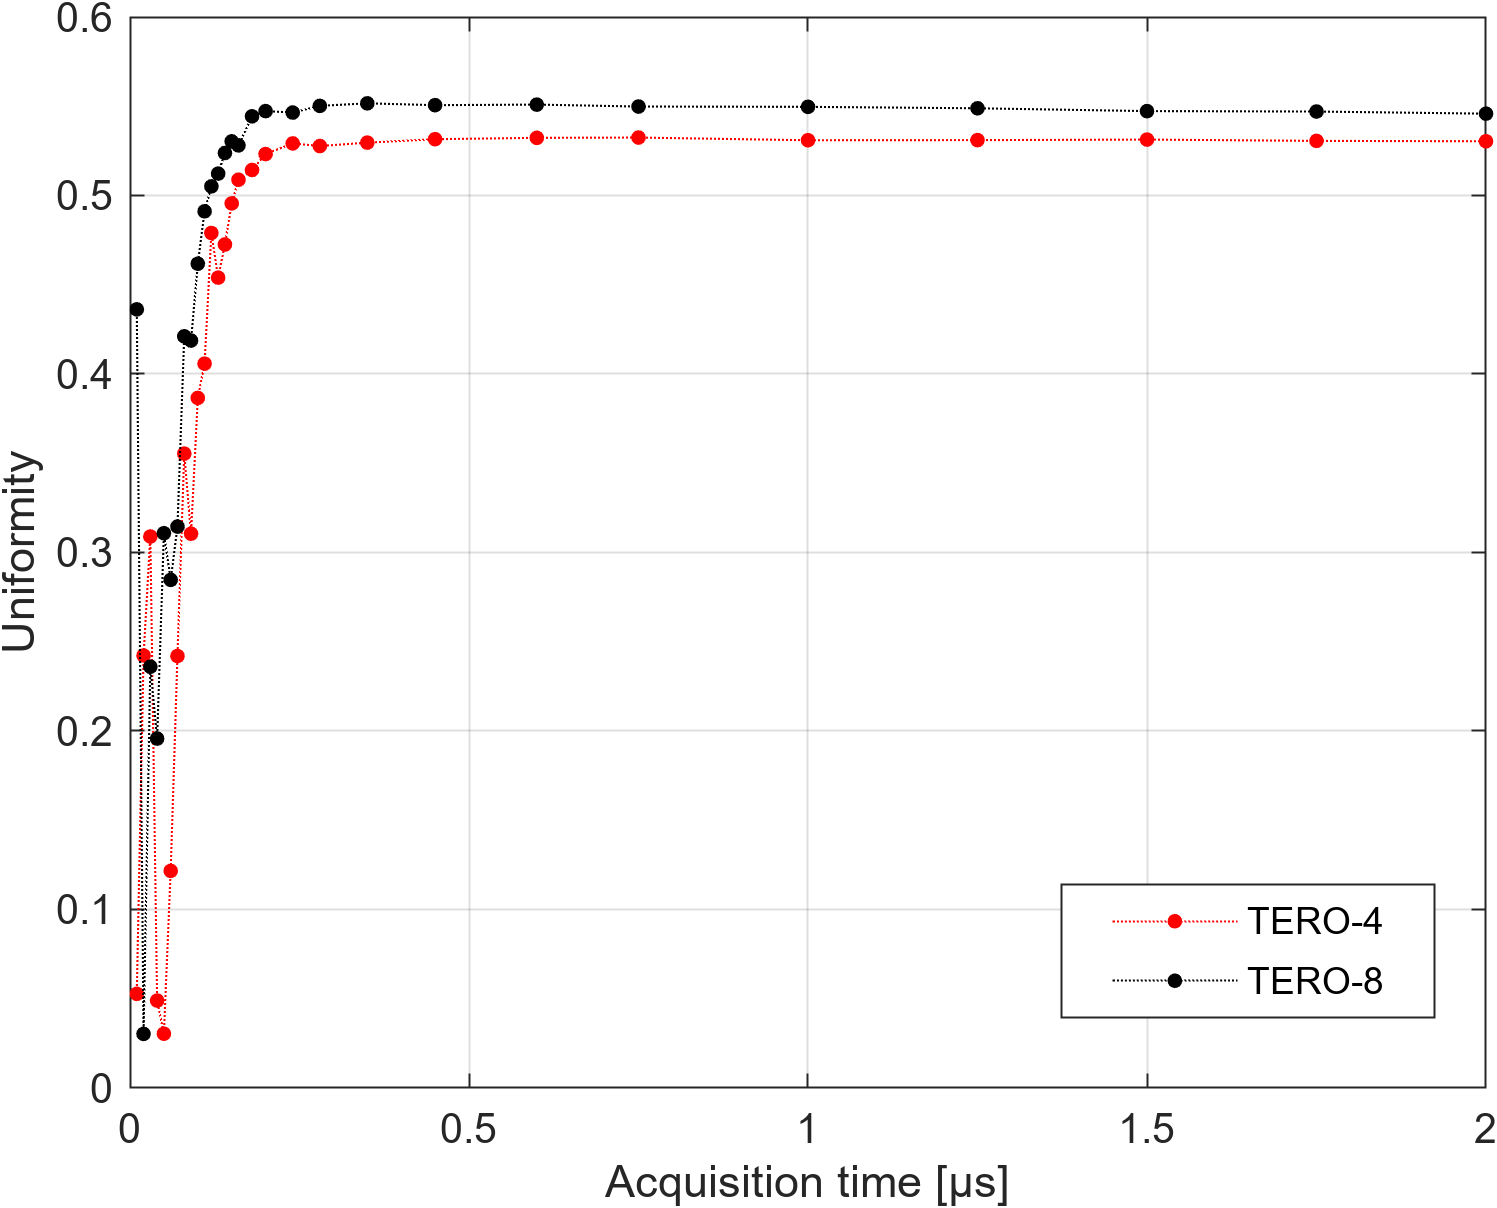
\includegraphics[width=\linewidth]
      {images/unlocked_tero_8_intra_uniformity.png}
      \subcaption{Uniformity}
   \end{minipage}\hfill
   \begin{minipage}[b]{0.50\linewidth}   
      \centering 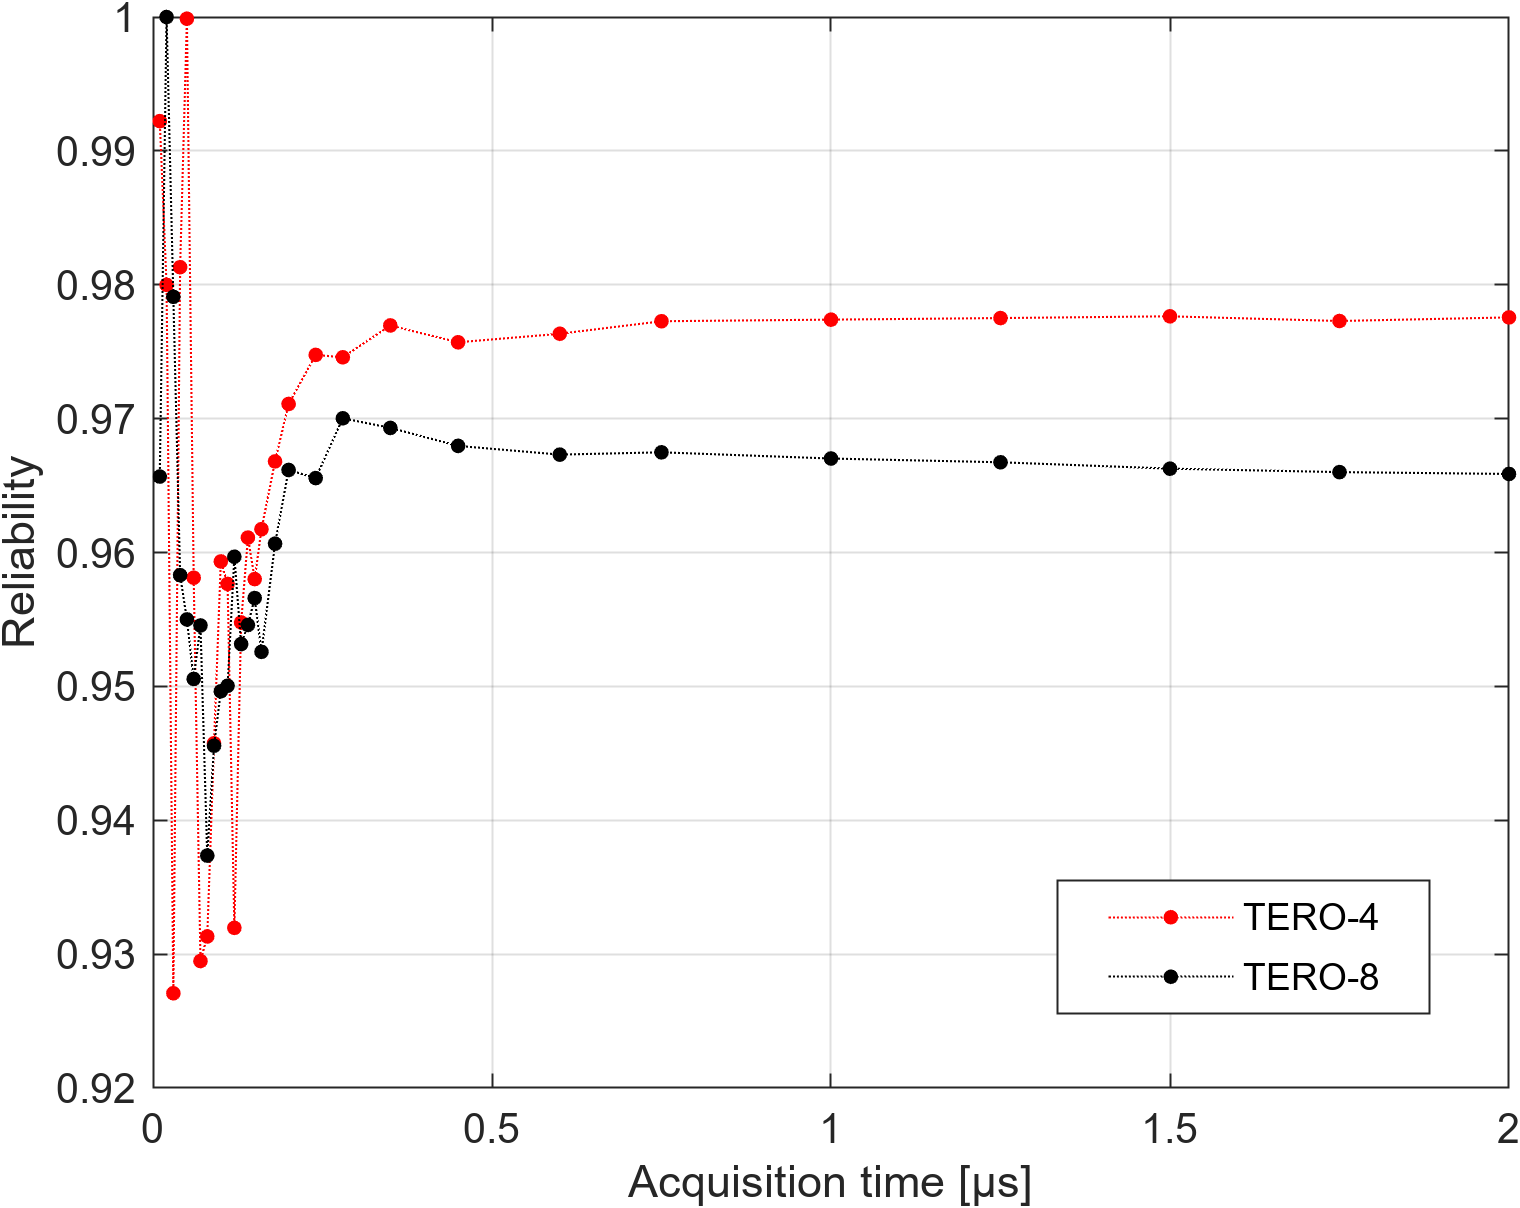
\includegraphics[width=\linewidth]{images/unlocked_tero_8_intra_reliability.png}
      \subcaption{Reliability}
   \end{minipage}
   \caption{\label{fig:locked_improvement_tero_8}TERO-8 performance improvement using locked pin}
\end{figure}

\newpage
\section{LSFR combinations distribution}
\label{appendix:lsfr}

The LSFR is used to generate the combinations of cells to compare instead of storing them in memory. It ensures that all the combinations are covered exactly once except the '0-0' combination never generated, providing a uniform usage of each cell. However, this does not ensure that the cell usage stays as uniform as possible during the generation process, and it can be seen in figure~\ref{fig:cell_occurence} that it is indeed not completely uniform when only a part of the combination is generated. 


\begin{figure}[H]
    \centering
    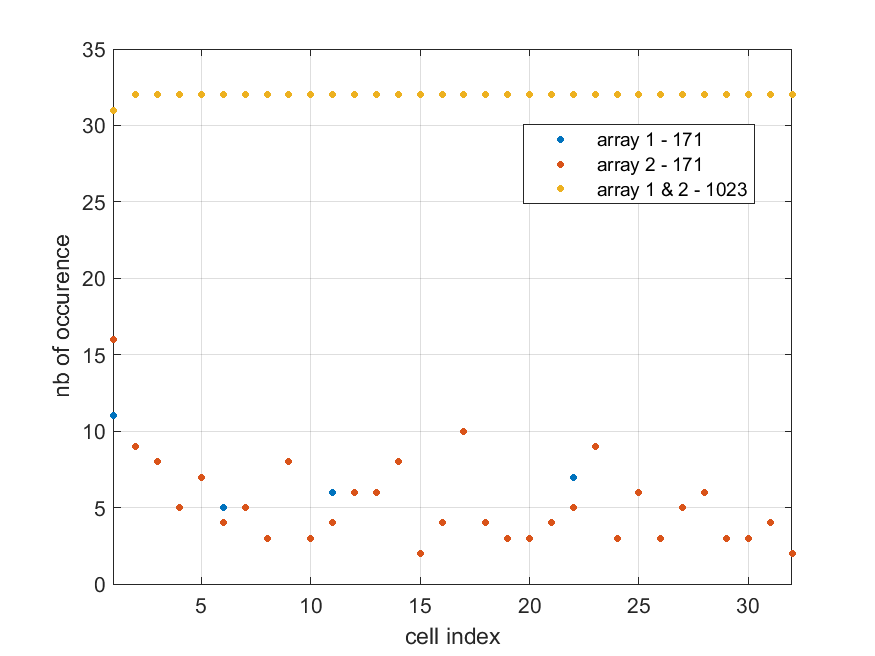
\includegraphics[width=0.7\linewidth]{images/cell_occurence_171.png}
    \caption{LSFR10 cells selection for only 171 bits}
    \label{fig:cell_occurence}
\end{figure}

This means that some cells are more used than others for comparison in this case. If those cells have an extreme final state (high or low number of oscillations in regard to the other), the comparisons with those cells will almost always generate the same bit. Since this cell is used more often, this could have a negative impact on the uniformity of the response.

\begin{table}[H]  
  \centering
    \begin{tabular}{|c|c|c|c|c|c|}
        \hline
        \textbf{TERO-8} & Response size & Uniformity & Reliability & Bit-aliasing & Uniqueness\\
        \hline
        Full & 1023 bits & 53.4\% & 97.6\% & 53.5\% & 49.4\%\\
        \hline
        Reduced & 171 bits & 53.4\% &97.7\% & 54.4\% & 49.9\%\\
        \hline
    \end{tabular}
   \caption{\label{tab:inter_perf_full_vs_reduce}TERO-8 performances for full and reduced response}
\end{table}

However, as we can see on the table~\ref{tab:inter_perf_full_vs_reduce}, this does not seem to have a significant impact on average on the TERO-8 implementation.

\newpage
\section{Python module}
\label{appendix:python_mod}

A Python module has been written to implement the UART interfaces in an easy-to-use method way. It used the \textbf{Pyserial} package for UART communication and \textbf{Numpy} to retrieve the data.

The PUF device is represented by the \textbf{PUF} class, which requires the port for the UART to be instantiated. We can also specify the baudrate and the initial value for the reference counter (to select the acquisition time).\\

Each interface with the PUF corresponds to a method:

\begin{itemize}
    \item \textbf{set\_ref\_limit(limit: int)}: update the limit of the reference counter, to change the acquisition time. The possible values are [1 -> 65536].
    \item \textbf{read\_raw()}: return the raw PUF response (1023 bits).
    \item \textbf{read\_ecc()}: return the PUF response after the BCH decoder (171 bits). The syndrome needs to be previously set using \textbf{set\_syndrome(syndrome: str)}.
    \item \textbf{read\_sha()}: return the sha256 key (256 bits).
\end{itemize}


For each reading operation, a second method has been created to easily record multiple samples for the same test. The return of those methods has their own class \textbf{SamplesReturnData} that stores the responses samples and computes the corresponding reference response and uniformity. This could easily be extended to also compute the reliability.

A second point that could be improved would be to compute the syndrome from the raw PUF response directly on this module instead of using Matlab. It could therefore automatically do the provision step at start then send the syndrome each time it is needed.



